
\chapter{Welcome to EMEP }

This guide gives a brief documentation of the EMEP/MSC-W model
version rv4.8. 
It is intended primarily as a guide on how to run the model, and
to help users wishing to understand or change 
the model in terms of domains, outputs, chemistry, etc.


The main documentation for the EMEP/MSC-W model is an article pulished 
in Atmospheric Chemistry and Physics in 2012. 
This article will be referred to as Simpson et al. (2012) in
this manual. 


\begin{itemize}
\item
Simpson, D., Benedictow, A., Berge, H., Bergstr\"om, R., Emberson, L.D., Fagerli, H., Flechard, C.R., Hayman, G.D., Gauss, M., Jonson, J.E., Jenkin, M.W., Ny\'iri, \'A, Richter, C., Semeena, V.S, Tsyro, S., Tuovinen, J.-P., Valdebenito, \'A., and Wind, P.:
The EMEP MSC-W chemical transport model – technical description.  
Atmospheric Chemistry and Physics, 12, 7825-7865, 2012.\\
\url{http://www.atmos-chem-phys.net/12/7825/2012/acp-12-7825-2012.html}
\end{itemize}


The model source code is available from the EMEP/MSC-W Open Source website:\\ 
\url{https://wiki.met.no/emep/page1/emepmscw_opensource}

\newpage

\section{Licenses and Caveats}

The EMEP code is provided under the GNU General Public License version 3
(\url{http://fsf.org} and/or
\url{http://www.gnu.org/copyleft/gpl.html}).

Each code module is prefaced with something like:
\begin{quote}
\begin{small}
\begin{verbatim}
! <EXAMPLE_CODE.f90 - A component of the EMEP MSC-W  Eulerian
!          Chemical transport Model>
!*****************************************************************************!
!*
!*  Copyright (C) 2007-2012 met.no
!*
!*  Contact information:
!*  Norwegian Meteorological Institute
!*  Box 43 Blindern
!*  0313 OSLO
!*  NORWAY
!*  email: emep.mscw@met.no
!*
!*    This program is free software: you can redistribute it and/or modify
!*    it under the terms of the GNU General Public License as published by
!*    the Free Software Foundation, either version 3 of the License, or
!*    (at your option) any later version.
!*
!*    This program is distributed in the hope that it will be useful,
!*    but WITHOUT ANY WARRANTY; without even the implied warranty of
!*    MERCHANTABILITY or FITNESS FOR A PARTICULAR PURPOSE.  See the
!*    GNU General Public License for more details.
!*
!*    You should have received a copy of the GNU General Public License
!*    along with this program.  If not, see <http://www.gnu.org/licenses/>.
!*****************************************************************************!
\end{verbatim}
\end{small}
\end{quote}
And a copy of the license file, {\bf gpl.txt}, is provided with the
model code source files.

\noindent It is important to note that the code is provided ``as it is'', 
and EMEP/MSC-W has very limited resources with which to support
code-usage. 

%% To help users an {\bf EMEP Forum} is available from the
%% EMEP/MSC-W Open Source website in section ``Users'': ``EMEP Forum''. 
%% Support to the user community will develop here with your contribution. 
%% Please let us know what your needs for information are 
%% (e-mail: emep.mscw@met.no).

\newpage

\section{Computer Information}
\label{sec:compinf}

To compile the EMEP/MSC-W model you need:\\

\textbf{Fortran 95 compiler}

\textbf{NetCDF Library ($>$4.1.3)}

\textbf{MPI Library ($>$1.0)}\\

It is necessary to compile with double precision reals (8 bytes
reals). The program has been used on computers ranging from a Linux laptop to supercomputers 
(Itanium2 cluster, Intel Xeon cluster, Cray XT4, IBM power5+). It is compatible with all 
compilers tested so far:  Intel, PGI, gfortran, XL fortran. A Makefile is included,  
the path to netcdf (INCL and LLIB) have to be adapted to your machine, and the fortran 
compiler (F90) and flags (F90FLAGS) to the compiler you are using.



The code has been tested with 1 to 1024 CPUs, and scales well (for large grids).  If only one 
CPU is used 1-2 GB memory is required. If more than one,
for example 64 CPUs are used, 200 MB of memory per CPU is enough (in
the case of a 132 X 159 grid size). For runs on more than 32 CPUs, a fast interconnect is 
recommended (infiniband for example), for smaller runs, gigabit ethernet is sufficient. 
It takes $\sim$ 5 hrs on 64*Xeon X5355 (2.66GHz) for 1 year simulation.

When downloading input data in order to do a ``base run'' please make
sure that there are 35 Gb disc space available, especially due to
large meteorology input files. The model can be run for shorter periods, users 
can download meteorology for only the period they are interested in, pluss one day. 
 

\section{Getting Started}


It is recommended to read all the chapters of this EMEP/MSC-W model
User Guide before you start downloading anything from the EMEP/MSC-W Open
Source website.

%% Please register as an EMEP User on the {\bf EMEP Forum}
%% (EMEP/MSC-W Open Source website under ``Users'' section: ``EMEP Forum'')
%% before you start downloading the EMEP/MSC-W model code and/or input
%% data. This will give you access to further communication with the
%% developing team and to the section on ``Questions and Answers''. 


This is what you need to do before you can do a ``base run'' with the 
EMEP/MSC-W model:

\begin{itemize}
%\item Register as an EMEP User
\item Read the EMEP/MSC-W model User Guide
\item
Download input data (description in Chapter~\ref{ch:InputFiles} and
data available from the EMEP/MSC-W Open Source website under ``Download''
section: ``Input Data'')
\item
Download the EMEP/MSC-W model source code (description in 
section~\ref{sec:ModelCode} and the files are available from the EMEP/MSC-W 
Open Source website under ``Download'' section: ``Model Code'')
\item
Follow the instructions for 'Submitting a Run' description in
Chapter~\ref{ch:SubmitARun}.
\item
Download some model results for comparison, description in
Chapter~\ref{ch:output} and the files are available from the EMEP/MSC-W 
Open Source website under ``Download'' section: ``Model Results''. 
%NEWTOOLS:
% \item
% If wanted, download some helper programmes to read site and sonde outputs, 
% see sections~\ref{sec:tools},\ref{sec:sitesonde}.
% The files are available from the EMEP
% Open Source website under ``Download'' section: ``Tools''.


\end{itemize}

\section{Model code}
\label{sec:ModelCode}

The EMEP/MSC-W model code version rv.4.8 are archived as a tar file. 
The tar file is called ``EMEP\_MSC-W\_model.rv4.8.OpenSource.tar.gz'' and 
is downloadable from the EMEP/MSC-W Open Source website.

Once this file is untarred all model files needed for a model run will be 
found under the directory \\ {\bf EMEP\_MSC-W\_model.rv4.8.OpenSource/code/} 
where the model source code, makefiles, and a copy of the license file are 
stored. An overview is given in Table~\ref{Tab:modelfiles}

\begin{table}[h]
\begin{center}
\caption{Contents of ``EMEP\_MSC-W\_model.rv4.8.OpenSource.tar'' file
   \label{Tab:modelfiles}}
\begin{tabular}{ll}
& \\
\hline
Type      & Filename          \\
\hline
& \\
{\bf Model code directory} & EMEP\_MSC-W\_model.rv4.8.OpenSource/code \\ 
\hline
modules files & *.f90 \\
include files & *.inc \\
namelist & config\_emep.nml \\
makefiles & Makefile and Makefile.SRCS \\
dependency file &  dependencies\\
a copy of the license & gpl.txt \\
\hline
\end{tabular}
\end{center}
\end{table}

In addition there is a run script called ``modrun.sh'', which will be placed 
in the \\{\bf EMEP\_MSC-W\_model.rv4.8.OpenSource/}  directory. The run 
script, ``modrun.sh'', can easily be modified to work on your computer system. 
This script is described in detail in Chapter \ref{ch:SubmitARun}. 
 
%NEWTOOLS
% \section{Helper tools}
% \label{sec:tools}
% ????
% For users interested in reading the ascii site and sonde specific outputs,
% two help programmes (Rd\_sites.f90, Rd\_sondes.f90) are provided, 
% in the \\{\bf EMEP\_Unified\_model.OpenSource2012/tools}  directory. These
% programmes are readily compiled with e.g. gfortran, and can be run without
% arguments to obtain usage instructions. See section~\ref{sec:sitesonde}
% for more details.


\section{Model grid}
\label{sec:ModelGrid}

The current EMEP model version, and the provided gridded input data,
have a horizontal resolution of 50$\times$50 km$^2$ (at 60$^\circ$N)
and are defined on a
polar stereographic projection with 20 sigma levels vertically. 
The model is very flexible with regard to the horizontal
resolution, in that it readily makes use of 
meteorological data provided with the model. The vertical
resolution is currently still restricted to the fixed 20 layer
system. The physical
description is given in detail in Chapter 2 of the EMEP Status Report
1/2003 Part I (Simpson {\sl et al.}, 2003).

In 2008 the official EMEP domain was extended eastwards in order to include the 
EECCA countries in the EMEP model grid, see Figure \ref{fig:EECCA}. To distinguish the new grid from the old EMEP 
grid, the new grid is called EECCA in this text and in the config\_emep.nml.

\begin{figure}[ht]
 \centering
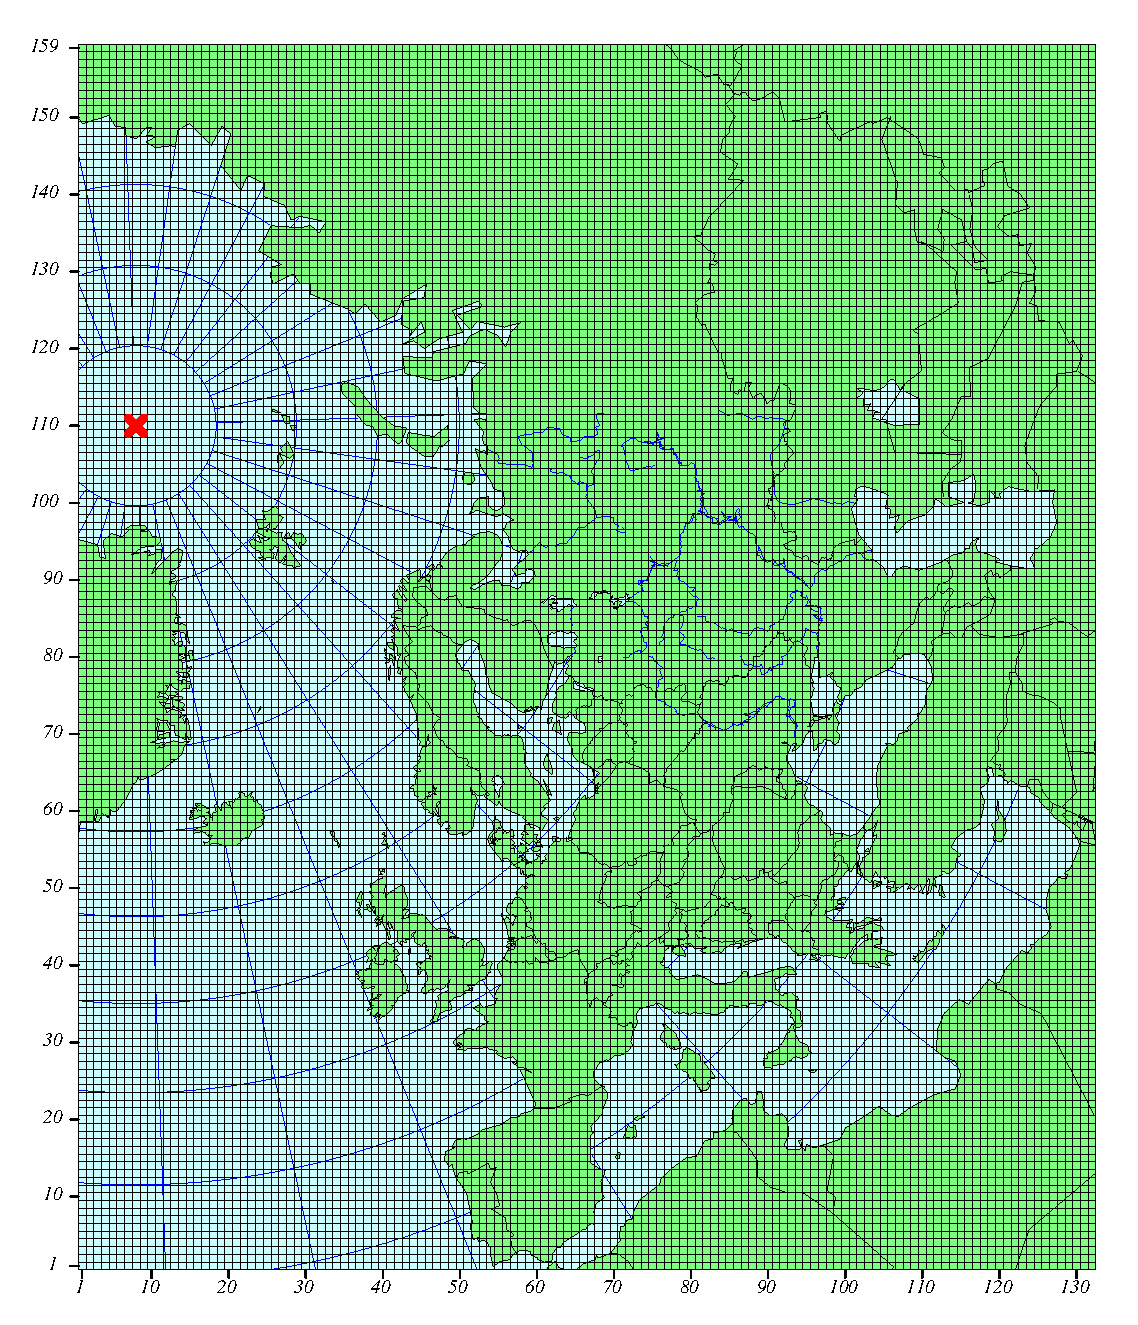
\includegraphics[scale=0.7]{EECCA.eps}
\caption{The extended EMEP grid covering EECCA area with
132$\times$159 gridpoints on 50$\times$50 km$^2$ resolution defined on a polarstereographic
projection.}\label{fig:EECCA}
\end{figure}


